\section{ESLs - \name{} Scheduling Libraries}   % Pronounced "Easel"
\label{sec:esl}

%Describe the problem - application code and programmer must deal with cumbersome resource management
% Controlling task placement through direct manipulation of ephemeral resources can be burdensome for applications with conventional scheduling requirements. While ESCHER grants flexibility to applications to compose arbitrary scheduling policies through combinations of resource constraints, it requires applications to maintain resource state and handle low-level resource specification for tasks. This resource specification can become particularly intricate when multiple scheduling policies must be composed. Moreover, many applications, such as MapReduce\cite{mapreduce} and dataframe\cite{DevinMasters} processing, share common scheduling objectives and can have a shared policy implementation.
Controlling task placement through direct manipulation of ephemeral resources can be burdensome for applications with conventional scheduling requirements. While the ESCHER API grants flexibility to applications to compose arbitrary scheduling policies
%through combinations of resource constraints
, it requires applications to maintain ephemeral resource state and handle resource specification for tasks. % This resource specification can become particularly intricate when multiple scheduling policies must be composed. Moreover, many applications, such as MapReduce\cite{mapreduce} and dataframe\cite{DevinMasters} processing, share common scheduling objectives and can have a shared policy implementation.
To reduce the application complexity and delineate scheduling policies from the mechanisms to implement them, we propose ESCHER Scheduling Libraries (ESLs).

ESLs are similar in spirit to Library Operating Systems (LibOS,~\cite{Kaashoek:1997:APF:268998.266644}) in the Exokernel\cite{exokernel} design.
% Just like a Library OS acts as a simplifying layer encapsulating the complexity of direct resource management exposed by an Exokernel, ESLs promote clean design and enable scheduling policies to be shared across different applications on an ESCHER scheduler.
In the same way that a LibOS encapsulates the complexity of direct resource management exposed by an Exokernel, an ESL abstracts the policy implementation and enables sharing across different \name{} applications.
% ESLs promote clean design and code re-use by abstracting all ESCHER related resource state into a unified layer that can be shared with other applications.
Moreover, this design makes applications portable across different cluster frameworks, e.g., Ray vs. Kubernetes~(\Cref{sec:impl}), since ESLs separate the application policy from the application code.
Finally, ESLs can optionally protect applications from invalid specification of ephemeral resource requests by verifying the consistency of resource requests using the \lstinline{get_cluster_state} call before launching the task.

% \begin{figure}[ht]
%     \centering
%     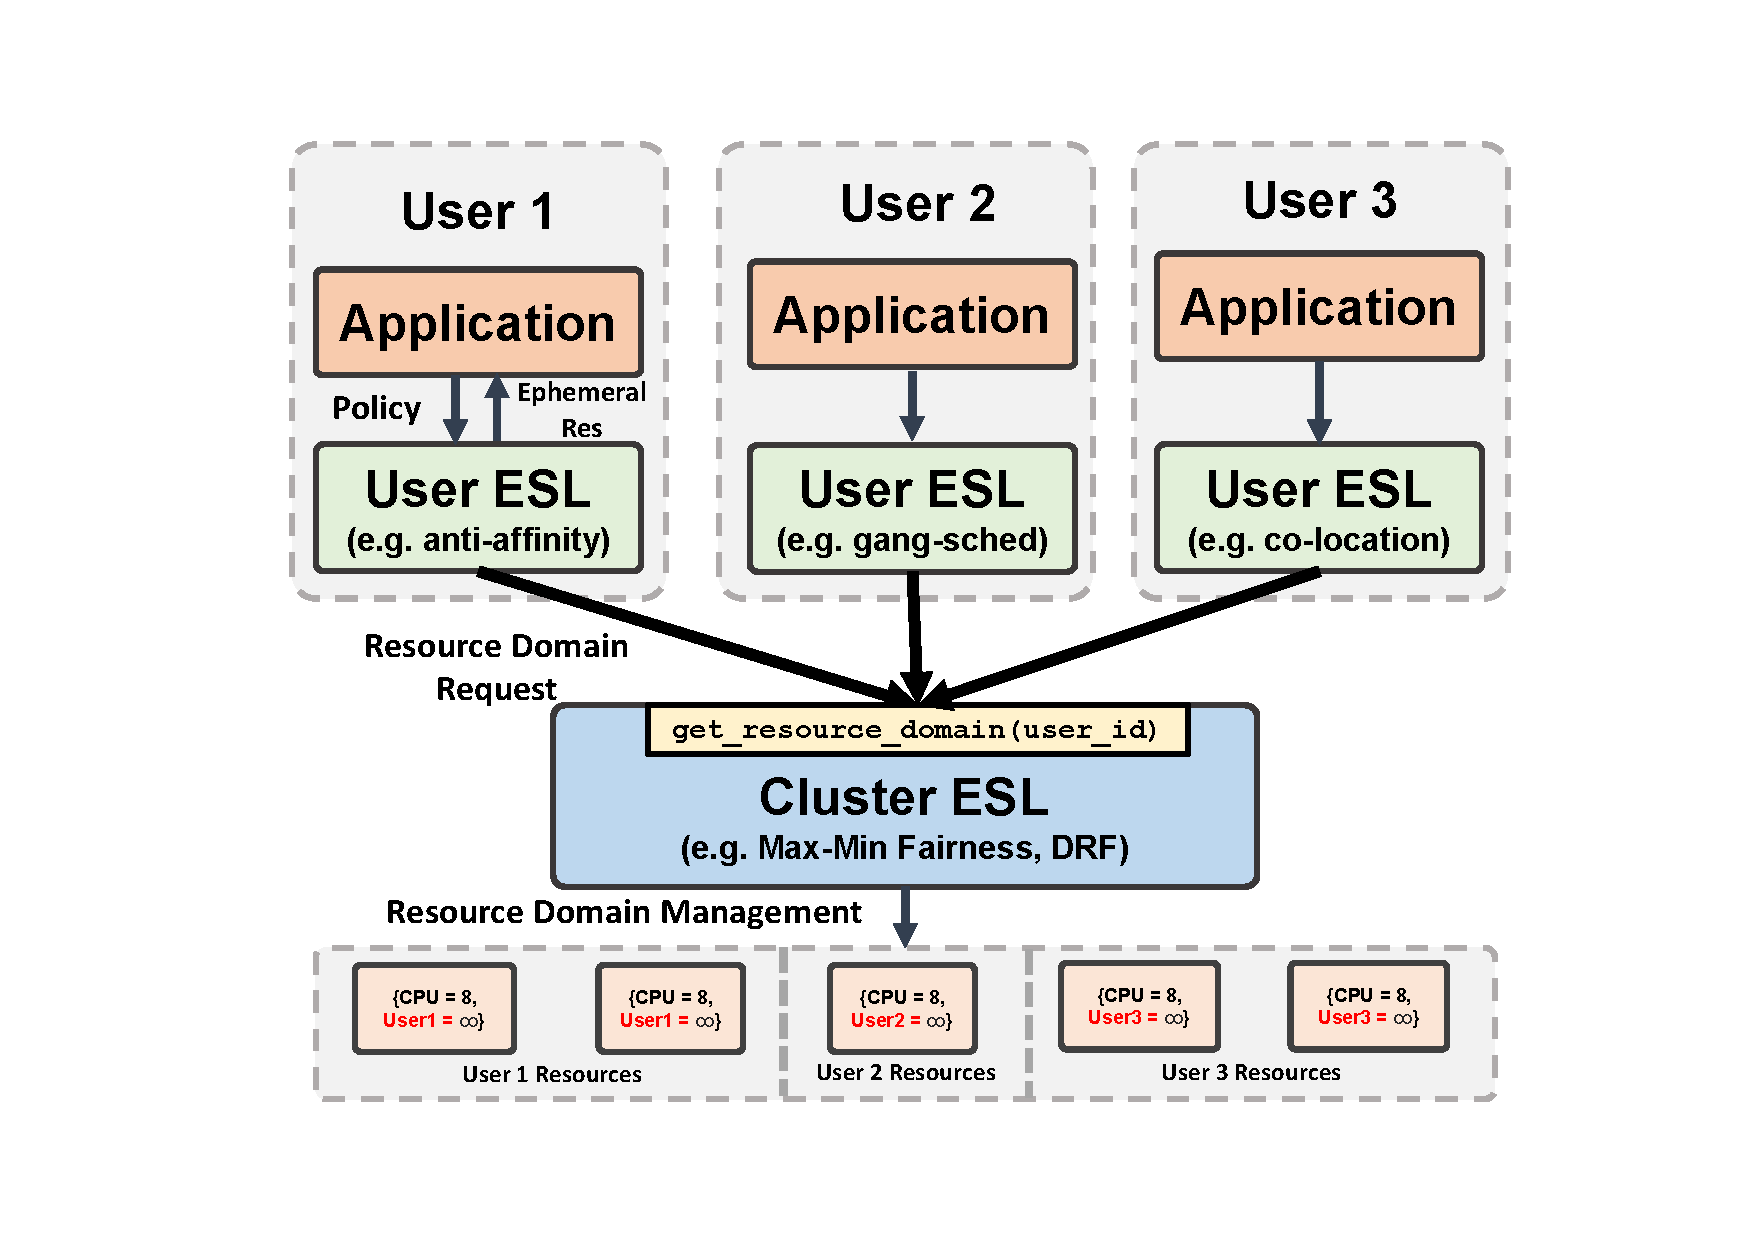
\includegraphics[width=\linewidth]{escher/figures/clusteresl_useresl.pdf}
%     \caption{
%         Isolation mechanisms in ESCHER. To avoid resource conflicts between ESLs, ESCHER uses a two-layer design to isolate applications. A cluster ESL provides a resource domain (a set of nodes) to each user's application-level ESLs. This resource domain is dynamically adjusted by the cluster ESL's policy. The resource domain restricts a user ESL from creating resources outside their authorized pool. 
%     }
%     \label{fig:esl-isolation}
%     %\vspace{-4mm}
% \end{figure}

\subsection{ESL Design}
An ESL encapsulates the state management for ephemeral resources and provides a unified API for implementing domain-specific scheduling policies. An application requests one of the many high level scheduling policies supported by an ESL, which then makes the appropriate ESCHER API calls and returns the exact resource specification the application should use to realize its desired policy. In our implementations, ESLs are designed as a daemon that can service scheduling requests made from a single or multiple applications.

 % Figure \ref{fig:esl-arch} describes the workflow to use an ESL. An application first initializes it or connects to a pre-existing ESL which implements the desired scheduling policy. It then makes a ESL specific call to select the policy and any related parameters (such as co-location group name, or minimum slots for gang scheduling). The ESL inspects the cluster state and invokes the \lstinline{set_resource()} API to update ephemeral resources if required. Finally, it returns the exact resource specification the task must use to satisfy the requested policy. This resource specification can be used as-is or further concatenated with with other resource specifications to compose custom policies.

Since distributed applications can have widely varying scheduling requirements, we anticipate the development of domain-specific ESLs which can strike a balance between generality and preserving low-level domain-specific optimizations. For instance, an ESL for dataframe processing applications could support data locality and task co-location, while adding implicit data-replication at the ESL layer to improve data locality. 

% Design - Explain the figure and how applications still have resource control if required. 2 Phase protocol for task submission.
\begin{sloppypar}
As an example, we illustrate a big-data ESL to encapsulate two popular policies --- data locality and task co-location. This ESL exposes two methods to applications: \lstinline[breaklines=true]{get_coloc_group(group_name, node_resources)} and \lstinline[breaklines=true]{get_dataloc_group(data_id)}. 
%\swang{no reference to get\_dataloc\_group in the listing?} fixed.
These methods allow an application to create logical locality groups in the ESL and get the resource specification which would place tasks in locality group. Internally, ESL maintains the state related to locality groups and implements the policies as described in Section \ref{policies}. Listing \ref{listing:eslexample} illustrates how an application interacts with the big-data ESL.
\end{sloppypar}

\begin{listing}
\begin{minted}{python}
esl = BigDataESL()
coloc_res = esl.get_colocation_group("mygroup", node_resources={gpu: 8})
dataloc_res = esl.get_dataloc_group(data_handle)

# Use ESL resource specification to co-locate tasks t1 and t2
# and enforce data locality for t3
t1.launch(resources+=coloc_res)
t2.launch(resources+=coloc_res)
t3.launch(resources+=dataloc_res)
\end{minted}
\caption{Using the big-data ESL to enforce task co-location. The ESL methods return a resource specification which is used to launch the co-located tasks.}
\label{listing:eslexample}
\end{listing}

% Comments - we anticipate domain specific scheduling libraries. ESLs are optional. 

% Benefits - Simplified application code, code resuse across applications, portability of applications, domain specific optimizations
% Moreover, using ESLs has four key benefits.
% \begin{itemize}
%     \item\textbf{Simplified Code:} The use of ESLs greatly simplifies application-level code since all ESCHER related resource state management is abstracted into a unified layer. 
%     \item\textbf{Code Re-use:} Applications performing similar tasks often have overlapping scheduling requirements. For instance, it is common for dataframe processing applications to require data locality. Instead of individually implementing data locality, all these applications could use instances a single ESL.
%     \item\textbf{Portability:} Exporting the policy implementation to the ESL makes applications portable across different cluster frameworks (such as Ray, Kubernetes) and updates to policy implementation can be pushed without affecting the application code.
%     \item\textbf{Resource specification safety:} Invalid specification of ephemeral resources due to stale resource state can render tasks unschedulable. ESLs can integrate resource safety checks which verify the consistency of resource requests using the \lstinline{get_cluster_state} call before launching the task.
%     %\item\textbf{Domain Specific Optimizations:} The use of ESLs allows domain specific optimizations like replication for datalocality
% \end{itemize}


\subsection{Fault tolerance}
\label{sec:esl-faulttol}
In the event of a node failure, ESCHER works in tandem with the fault-tolerance scheme of the underlying framework but also allows the application developers to specify custom fault-tolerance routines through an ESL. Most frameworks, including Ray\cite{ray} and Kubernetes\cite{kubernetes}, simply re-execute the tasks with the same resource requirement. However, since these resource requests include ephemeral resources which no longer exist, these re-executed tasks cannot be scheduled.

At the bare minimum, an ESL must ensure that ephemeral resources are restored at some other eligible node. To do this, ESCHER relies on the cluster framework to report failed nodes through the \lstinline{get_cluster_state} API. Once failed nodes are detected, an ESL can recreate the ephemeral resources on suitable nodes by replaying the \lstinline{set_resource} calls for the failed resources. If a candidate node is found, the resource is recreated, else the tasks must wait for the failed node to recover before they can be rescheduled. When a node is restored, it's resources are also reinitialized allowing any waiting tasks to get rescheduled. In addition to this basic policy, ESLs can define custom routines such as error reporting and logging after the ephemeral resources are restored.